\documentclass[border=5pt]{standalone}
\usepackage{tkz-euclide}
\NewDocumentCommand{\tangentdraw}{ O{} O{} m m m m m}{%
    % #1: line tikz style
    % #2: point tikz style
        % #3: point A
        % #4: point B
    % #5: tangent point
    % #6: radius
    % #7: angle
    \tkzDrawSegment[magenta,thick,#1](#3,#4)
    \tkzDefPointWith[orthogonal normed,K=#6](#5,#4)
    \tkzGetPoint{O}
    \tkzDefPointBy[rotation= center O angle -#7](#5) \tkzGetPoint{arc1} 
    \tkzDefPointBy[rotation= center O angle +#7](#5) \tkzGetPoint{arc2}
    \tkzDrawArc[magenta,thick,#1](O,arc1)(arc2)\tkzDrawPoints[black,thick,#2](#5)
}
\begin{document}
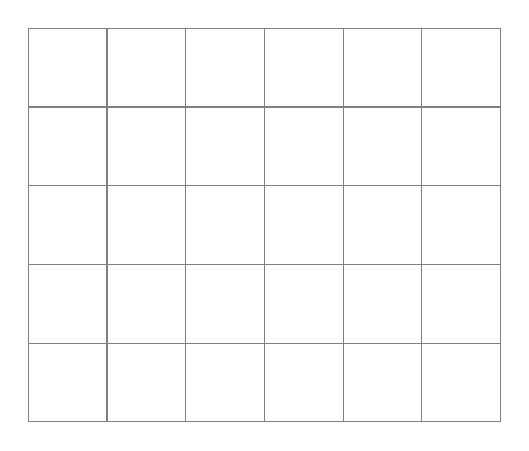
\begin{tikzpicture}
    \tkzInit[xmax=6, ymax=5]\tkzGrid
    \tkzDefPoints{0/4/A, 5/0/B}
    \tkzDefPointOnLine[pos=.67](A,B)\tkzGetPoint{P}
    \tangentdraw[][teal]{A}{B}{P}{6}{20}
\end{tikzpicture}
\end{document}